\documentclass{standalone}

\usepackage{tikz}

\begin{document}
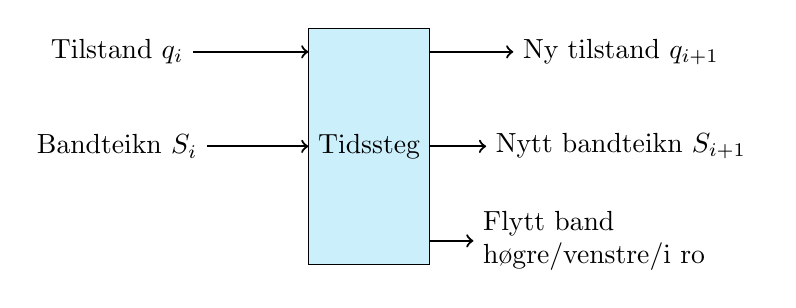
\begin{tikzpicture}
   \tikzstyle{every node}=[node distance=12mm]
   \node (qi) {Tilstand $q_i$} ;
   \node (si) [below of=qi] {Bandteikn $S_i$} ;
   \node (step) [draw,fill=cyan!20,right of=si,node distance=32mm,minimum height=30mm] {Tidssteg} ;

   \node (sj) [right of=step,node distance=32mm] {Nytt bandteikn $S_{i+1}$} ;
   \node (qj) [above of=sj] {Ny tilstand $q_{i+1}$} ;
   \node (mj) [below of=sj] {\parbox{35mm}{\raggedright Flytt band høgre/venstre/i ro}} ;

   \draw [thick,->] (qi.east) |- ([yshift=12mm]step.west) ;
   \draw [thick,->] (si.east) |- (step.west) ;
   \draw [thick,->] ([yshift=12mm]step.east) |- (qj.west) ;
   \draw [thick,->] (step.east) |- (sj.west) ;
   \draw [thick,->] ([yshift=-12mm]step.east) |- (mj.west) ;

\end{tikzpicture}
\end{document}
